%----------------------------------------------------------------------------------------
%	PACKAGES AND THEMES
%----------------------------------------------------------------------------------------
\documentclass[aspectratio=169,xcolor=dvipsnames,handout]{beamer}
\usetheme{Darmstadt}
\usecolortheme{seahorse}

\usepackage[hangul]{kotex}

\usepackage{hyperref}
\usepackage{amsfonts, amssymb}
\usepackage{graphicx} % Allows including images
\usepackage{booktabs, multicol, multirow} % Allows the use of \toprule, \midrule and \bottomrule in tables
\setbeamercovered{transparent}

\newcommand{\R}{\mathbb{R}}
\newcommand{\y}{\mathbf{y}}

%----------------------------------------------------------------------------------------
%	TITLE PAGE
%----------------------------------------------------------------------------------------

\title[한국의 불평등 현황]{한국의 불평등 현황} % The short title appears at the bottom of every slide, the full title is only on the title page
\subtitle{경제정의와 불평등}

\author[오성재]{오성재}

\institute[HNU] % Your institution as it will appear on the bottom of every slide, may be shorthand to save space
{
    한남대학교 \\
    탈메이지 교양학부 \\
}
\date{\today} % Date, can be changed to a custom date


%----------------------------------------------------------------------------------------
%	PRESENTATION SLIDES
%----------------------------------------------------------------------------------------

\begin{document}

\begin{frame}
    % Print the title page as the first slide
    \titlepage
\end{frame}

\begin{frame}{목차}
    \tableofcontents
\end{frame}
\section{한국의 불평등 현황}
\begin{frame}[<+->]
\frametitle{가계금융조사}
    \begin{itemize}
        \item 2012년부터 시작된 종단 자료.
        \item 자료의 종류 : 
        \begin{itemize}
            \item 횡단면(cross-section data) : 특정 집단, 특정 시점을 관측(올해 한남대 학생 신체검사 결과, 12월 1주차 정부지지도 등등).
            \item 시계열(time-series data) : 여러 집단, 한 시점을 관측(한국의 국민소득 추이, 주가지수 추이, 임기내 정부지지도 추이 등등).
            \item 종단연구(penal study or longitudinal study) : 특정 집단에 대하여 여러 시점을 추적 조사.
        \end{itemize}
        \item 표본설계 : 2015년 인구주택총조사 결과를 모집단으로 하는 전국 2만 가구 추출.
        \item 선정된 가구는 5년동안 조사.
    \end{itemize}
\end{frame}

\begin{frame}[<+->]
\frametitle{가계금융조사II}
    \begin{itemize}
        \item 조사항목
        \begin{itemize}
            \item 조사대상 가구의 자산, 부채, 소득, 지출 및 기타 인구 통계학적 특성.
            \item 가구소득 : 근로소득, 사업소득, 재산소득, 공적 이전소득, 사적 이전소득.
            \item 비소비지출 : 세금, 공적연금 기여금$\cdot$사회보험료, 가구간 이전지출, 비영리단체 이전지출, 이자비용 등.
        \end{itemize}
        \item 처분가능소득 : 가구소득 - 비소비지출.
        \item 균등화 처분가능소득 : 
        $$ \frac{ \text{처분가능소득}}{ \sqrt{\text{가구원수}}}.$$
        \item 상대적 빈곤율 : 전체 인구 중 균등화 처분가능 소득의 중위소득 50\% 이하인 가구가 차지하는 비율.
    \end{itemize}
\end{frame}

%------------------------------------------------

\begin{frame}[<+->]
    \begin{figure}
        \centering
        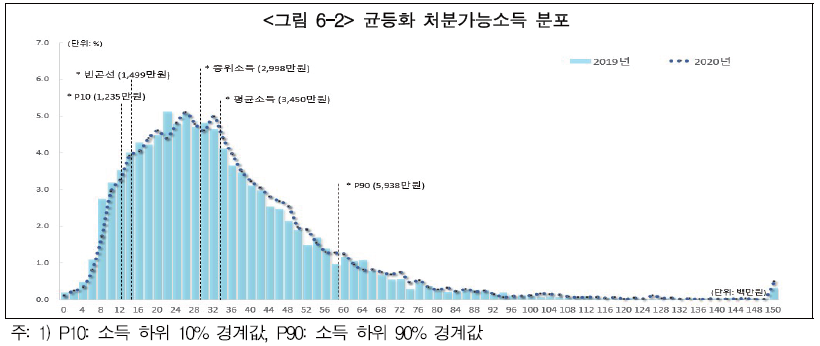
\includegraphics[width=.9\textwidth]{pic/incomedist.png}
    \end{figure}
\end{frame}
%------------------------------------------------

\begin{frame}[<+->]
    \begin{figure}
        \centering
        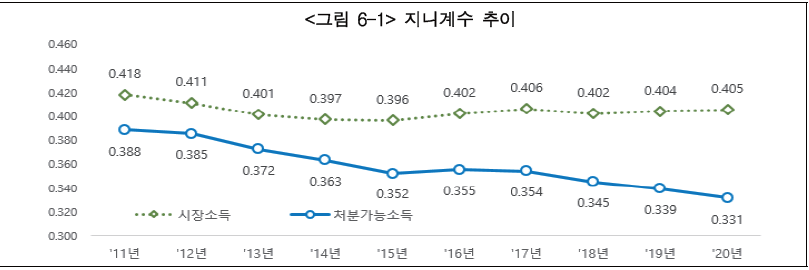
\includegraphics[width=.9\textwidth]{pic/gini_11-20.png}
    \end{figure}
    \begin{itemize}
        \item 한국의 가처분소득 불평등은 최근 10년간 하락세.
    \end{itemize}
\end{frame}
%------------------------------------------------

\begin{frame}[<+->]
    \begin{figure}
        \centering
        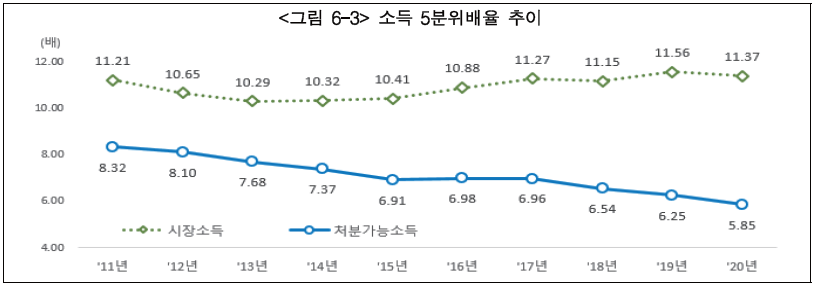
\includegraphics[width=.9\textwidth]{pic/1to5ratio.png}
    \end{figure}
    \begin{itemize}
        \item 상위소득계층과 하위소득계층 간의 격차 역시 하락.
    \end{itemize}
\end{frame}
%------------------------------------------------

\begin{frame}[<+->]
    \begin{figure}
        \centering
        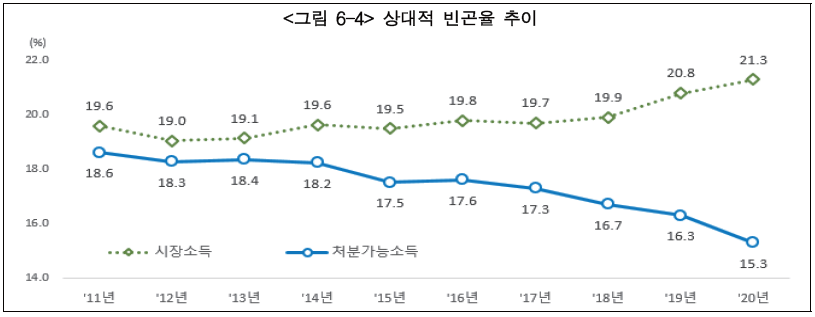
\includegraphics[width=.9\textwidth]{pic/relpov.png}
    \end{figure}
    \begin{itemize}
        \item 상대적 빈곤률 역시 하락하는 모양.
    \end{itemize}
\end{frame}
%------------------------------------------------
\begin{frame}[<+->]
    \begin{figure}
        \centering
        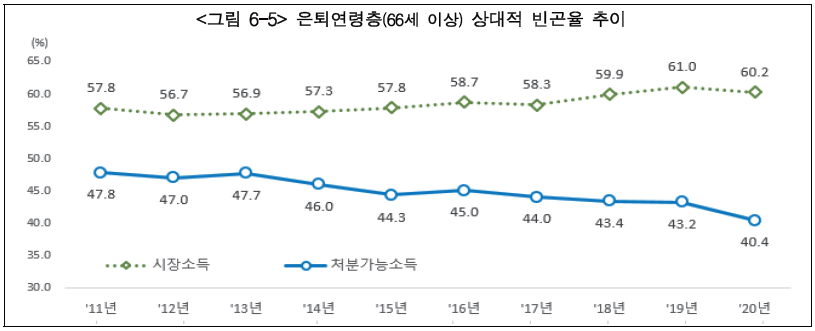
\includegraphics[width=.9\textwidth]{pic/agepov.png}
    \end{figure}
    \begin{itemize}
        \item 높은 노인빈곤률은 사회문제로 대두.
    \end{itemize}
\end{frame}
%------------------------------------------------
\end{document}